% Options for packages loaded elsewhere
\PassOptionsToPackage{unicode}{hyperref}
\PassOptionsToPackage{hyphens}{url}
%
\documentclass[
  9pt,
  ignorenonframetext,
]{beamer}
\usepackage{pgfpages}
\setbeamertemplate{caption}[numbered]
\setbeamertemplate{caption label separator}{: }
\setbeamercolor{caption name}{fg=normal text.fg}
\beamertemplatenavigationsymbolsempty
% Prevent slide breaks in the middle of a paragraph
\widowpenalties 1 10000
\raggedbottom
\setbeamertemplate{part page}{
  \centering
  \begin{beamercolorbox}[sep=16pt,center]{part title}
    \usebeamerfont{part title}\insertpart\par
  \end{beamercolorbox}
}
\setbeamertemplate{section page}{
  \centering
  \begin{beamercolorbox}[sep=12pt,center]{part title}
    \usebeamerfont{section title}\insertsection\par
  \end{beamercolorbox}
}
\setbeamertemplate{subsection page}{
  \centering
  \begin{beamercolorbox}[sep=8pt,center]{part title}
    \usebeamerfont{subsection title}\insertsubsection\par
  \end{beamercolorbox}
}
\AtBeginPart{
  \frame{\partpage}
}
\AtBeginSection{
  \ifbibliography
  \else
    \frame{\sectionpage}
  \fi
}
\AtBeginSubsection{
  \frame{\subsectionpage}
}
\usepackage{amsmath,amssymb}
\usepackage{lmodern}
\usepackage{iftex}
\ifPDFTeX
  \usepackage[T1]{fontenc}
  \usepackage[utf8]{inputenc}
  \usepackage{textcomp} % provide euro and other symbols
\else % if luatex or xetex
  \usepackage{unicode-math}
  \defaultfontfeatures{Scale=MatchLowercase}
  \defaultfontfeatures[\rmfamily]{Ligatures=TeX,Scale=1}
\fi
\usetheme[]{Frankfurt}
\usecolortheme{beaver}
% Use upquote if available, for straight quotes in verbatim environments
\IfFileExists{upquote.sty}{\usepackage{upquote}}{}
\IfFileExists{microtype.sty}{% use microtype if available
  \usepackage[]{microtype}
  \UseMicrotypeSet[protrusion]{basicmath} % disable protrusion for tt fonts
}{}
\makeatletter
\@ifundefined{KOMAClassName}{% if non-KOMA class
  \IfFileExists{parskip.sty}{%
    \usepackage{parskip}
  }{% else
    \setlength{\parindent}{0pt}
    \setlength{\parskip}{6pt plus 2pt minus 1pt}}
}{% if KOMA class
  \KOMAoptions{parskip=half}}
\makeatother
\usepackage{xcolor}
\IfFileExists{xurl.sty}{\usepackage{xurl}}{} % add URL line breaks if available
\IfFileExists{bookmark.sty}{\usepackage{bookmark}}{\usepackage{hyperref}}
\hypersetup{
  pdfauthor={Marcel Guzik},
  hidelinks,
  pdfcreator={LaTeX via pandoc}}
\urlstyle{same} % disable monospaced font for URLs
\newif\ifbibliography
\usepackage{listings}
\newcommand{\passthrough}[1]{#1}
\lstset{defaultdialect=[5.3]Lua}
\lstset{defaultdialect=[x86masm]Assembler}
\usepackage{graphicx}
\makeatletter
\def\maxwidth{\ifdim\Gin@nat@width>\linewidth\linewidth\else\Gin@nat@width\fi}
\def\maxheight{\ifdim\Gin@nat@height>\textheight\textheight\else\Gin@nat@height\fi}
\makeatother
% Scale images if necessary, so that they will not overflow the page
% margins by default, and it is still possible to overwrite the defaults
% using explicit options in \includegraphics[width, height, ...]{}
\setkeys{Gin}{width=\maxwidth,height=\maxheight,keepaspectratio}
% Set default figure placement to htbp
\makeatletter
\def\fps@figure{htbp}
\makeatother
\setlength{\emergencystretch}{3em} % prevent overfull lines
\providecommand{\tightlist}{%
  \setlength{\itemsep}{0pt}\setlength{\parskip}{0pt}}
\setcounter{secnumdepth}{-\maxdimen} % remove section numbering
\ifLuaTeX
  \usepackage{selnolig}  % disable illegal ligatures
\fi

\title{Rust Presentation}
\author{Marcel Guzik}
\date{}

\begin{document}
\frame{\titlepage}

\hypertarget{why-rust}{%
\section{Why Rust}\label{why-rust}}

\begin{frame}{Why Rust}
\begin{itemize}
\item
  \textbf{Both safe and performant. No tradeoffs.}
\item
  Zero cost abstractions!

  Really?

  \href{https://pkolaczk.github.io/overhead-of-optional/}{Really!}
\item
  Both low-level and high-level

  Write mostly high-level code, go low-level when you need it!
\end{itemize}
\end{frame}

\begin{frame}
\begin{itemize}
\item
  Memory safety

  Eliminate entire classes of bugs at compile time! You \textbf{can't}
  corrupt memory when using safe Rust!

  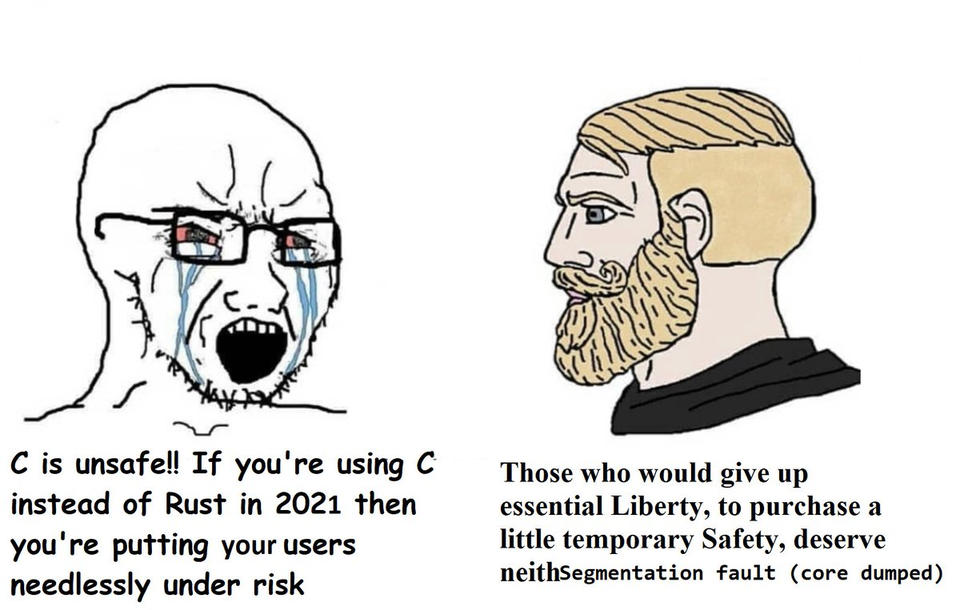
\includegraphics{img/memorysafety.jpg}
\end{itemize}
\end{frame}

\begin{frame}
\begin{itemize}
\item
  Good tooling and helpful compiler

  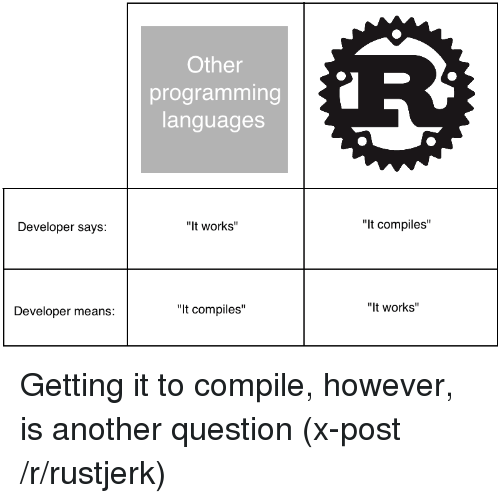
\includegraphics[width=0.5\textwidth,height=\textheight]{img/it_compiles_it_works.png}
\end{itemize}
\end{frame}

\begin{frame}
Rust's focus on safety famously makes implementing classical data
structures more difficult, eg. writing a linked list is challenging for
a beginner.

https://rust-unofficial.github.io/too-many-lists/
\end{frame}

\hypertarget{borrow-checking}{%
\subsection{Borrow checking}\label{borrow-checking}}

\begin{frame}{Move semantics}
\protect\hypertarget{move-semantics}{}
Move semantics in Rust are better than in C++. Why?

https://www.thecodedmessage.com/posts/cpp-move/

Short version:

In Rust, if the object is moved, it can't be accessed anymore

In C++, the moved object is still accessible, but is ``empty'', you need
to explicitly handle that case in the destructor, therefore move
semantics are not zero cost
\end{frame}

\hypertarget{rich-type-system}{%
\subsection{Rich type system}\label{rich-type-system}}

\begin{frame}{Rich type system}
\begin{itemize}
\tightlist
\item
  Algebraic Data Types
\item
  Generics
\item
  Traits
\end{itemize}
\end{frame}

\begin{frame}{Traits}
\protect\hypertarget{traits}{}
\begin{figure}
\centering

\includegraphics[width=0.5\textwidth,height=\textheight]{img/traits.jpg}
\caption{traits}
\end{figure}
\end{frame}

\begin{frame}
Traits are like interfaces from Java or Go, but better.

\begin{itemize}
\tightlist
\item
  https://softwareengineering.stackexchange.com/questions/247298/how-are-rust-traits-different-from-go-interfaces\#247313
\item
  https://stackoverflow.com/questions/69477460/is-rust-trait-the-same-as-java-interface
\end{itemize}
\end{frame}

\begin{frame}[fragile]
In short:

\begin{itemize}
\item
  it gives you a choice between static and dynamic dispatch (static
  dispatch means bigger code size but faster generics)

\begin{lstlisting}
// fast, bigger code size
fn static_dispatch<T: MyTrait>(arg: T) { }

// slow, less code size, uses Vtable
fn dynamic_dispatch(arg: Box<dyn MyTrait>) { }
\end{lstlisting}
\end{itemize}
\end{frame}

\begin{frame}[fragile]
\begin{itemize}
\item
  object definition / method implementation is decoupled (you implement
  in impl blocks)

\begin{lstlisting}
#[derive(Debug, Clone, Copy)]
struct Vec3 {
    x: f32,
    y: f32,
    z: f32,
}

impl Add for Vec3 {
    type Output = Vec3;

    fn add(self, rhs: Self) -> Self::Output {
        Vec3 {
            x: self.x + rhs.x,
            y: self.y + rhs.y,
            z: self.z + rhs.z,
        }
    }
}

impl Add<f32> for Vec3 {
    type Output = Vec3;

    fn add(self, rhs: f32) -> Self::Output {
        Vec3 {
            x: self.x + rhs,
            y: self.y + rhs,
            z: self.z + rhs,
        }
    }
}
\end{lstlisting}
\end{itemize}
\end{frame}

\begin{frame}[fragile]
\begin{itemize}
\item
  you can conditionally implement a trait for a type

\begin{lstlisting}
impl<T> Clone for Vec<T> where T: Clone {...}
\end{lstlisting}
\end{itemize}
\end{frame}

\begin{frame}[fragile]
\begin{itemize}
\item
  associated types, fuctions, values

\begin{lstlisting}
trait Iterator {
    type Item;
}

struct Iter<T>;
impl Iterator for Iter<T> {
    type Item = &T;
}

struct IterMut<T>;
impl Iterator for IterMut<T> {
    type Item = &mut T;
}

struct IntoIter<T>;
impl Iterator for IntoIter<T> {
    type Item = T;
}
\end{lstlisting}
\end{itemize}
\end{frame}

\begin{frame}[fragile]
\begin{block}{Most important standard library traits:}
\protect\hypertarget{most-important-standard-library-traits}{}
\begin{itemize}
\tightlist
\item
  Debug: Debug print formatting
\item
  Copy (requires Clone): Types that can be implicitly and trivially
  copied via bitwise copy
\item
  Clone: Types that can be explicitly cloned by calling
  \passthrough{\lstinline!.clone()!} on them.
\item
  Send: The type can be safely sent between threads
\item
  Sync: The type can be safely accessed via references from different
  threads. If \passthrough{\lstinline!\&T!} is
  \passthrough{\lstinline!Send!}, then \passthrough{\lstinline!Sync!} is
  derived automatically
\end{itemize}
\end{block}
\end{frame}

\begin{frame}
Comparing values:

\begin{itemize}
\tightlist
\item
  PartialEq: For types that have partial equality
\item
  Eq: For types that have full equality
\item
  PartialOrd: For types with partial ordering (type can be compared if
  its less, greater, or equal)
\item
  Ord: For types with total ordering (can be sorted)
\end{itemize}
\end{frame}

\begin{frame}[fragile]
Also:

\begin{itemize}
\item
  \passthrough{\lstinline!Sized!}: The size of this type is known at
  compile time. If the type has known size, it can be used as fields in
  structs or placed on the stack. \passthrough{\lstinline!?Sized!}
  (maybe sized) means size of type is not known at compile time.

  Unlike previous traits, this is assumed for all types, and only
  unsized types implement \passthrough{\lstinline"!Sized"} (not sized).
  Example:

  \begin{itemize}
  \tightlist
  \item
    https://doc.rust-lang.org/stable/std/primitive.slice.html\#impl-Sized
  \item
    https://doc.rust-lang.org/stable/std/primitive.str.html\#impl-Sized
  \end{itemize}

  Slices and string slices are not \passthrough{\lstinline!Sized!}, but
  the references to them are.
\end{itemize}
\end{frame}

\begin{frame}
\textbf{\href{https://fasterthanli.me/articles/aiming-for-correctness-with-types}{We
use rich type systems to design APIs that are flexible and simple, but
most importantly, correct.}}
\end{frame}

\hypertarget{algebraic-data-types}{%
\subsection{Algebraic data types}\label{algebraic-data-types}}

\begin{frame}{Algebraic data types}
What is algebraic data type?

\begin{quote}
In computer programming, especially functional programming and type
theory, an algebraic data type is a kind of composite type, i.e., a type
formed by combining other types.
\end{quote}

We can combine types in two ways:

\begin{itemize}
\tightlist
\item
  Sum types
\item
  Product types
\end{itemize}

In other languages, structs/classes are like a product type, but there
is no proper sum type.
\end{frame}

\begin{frame}[fragile]
In Rust, enums are sum types. Enums can contain values.

Example: standard library
\passthrough{\lstinline!Option!}/\passthrough{\lstinline!Result!} types.

\begin{lstlisting}
enum Option<T> {
    Some(T),
    None
}
\end{lstlisting}

\begin{lstlisting}
let some_int: Option<i32> = Some(5);
let no_int: Option<i32> = None;
\end{lstlisting}

\begin{lstlisting}
enum Result<T, E> {
    Ok(T),
    Err(E)
}
\end{lstlisting}

\begin{lstlisting}
// Returns string on success. Returns error code on failure.
fn op_that_can_fail -> Result<String, i32> {
    // ...
}

let result = op_that_can_fail();

match result {
    Ok(text) => println!("success: {text}"),
    Err(err_code) => println!("error! code: {err_code}")
}
\end{lstlisting}
\end{frame}

\begin{frame}[fragile]
It is impossible to not error check in Rust, because you need to handle
the error to access the success value:

\begin{lstlisting}
let text: String = std::fs::read_to_string("file.txt");
println!("{text}");
\end{lstlisting}

\begin{lstlisting}
error[E0308]: mismatched types
 --> examples/result.rs:2:24
  |
2 |     let text: String = std::fs::read_to_string("file.txt");
  |               ------   ^^^^^^^^^^^^^^^^^^^^^^^^^^^^^^^^^^^ expected struct `String`, found enum `Result`
  |               |
  |               expected due to this
  |
  = note: expected struct `String`
               found enum `Result<String, std::io::Error>`

For more information about this error, try `rustc --explain E0308`.
error: could not compile `rust-demo` due to previous error
\end{lstlisting}
\end{frame}

\begin{frame}[fragile]
To unwrap the value on success, but exit the program on failure, use
\passthrough{\lstinline!.unwrap()!} or
\passthrough{\lstinline!.expect("your message")!}.

\begin{lstlisting}
let text: String = std::fs::read_to_string("file.txt").unwrap();
println!("{text}");
\end{lstlisting}

On failure (eg. when \passthrough{\lstinline!file.txt!} does not exist):

\begin{lstlisting}
thread 'main' panicked at 'called `Result::unwrap()` on an `Err` value: Os { code: 2, kind: NotFound, message: "No such file or directory" }', examples/result.rs:2:60
note: run with `RUST_BACKTRACE=1` environment variable to display a backtrace
\end{lstlisting}
\end{frame}

\hypertarget{generics}{%
\subsection{Generics}\label{generics}}

\begin{frame}{Generics}
Trait based generics
\end{frame}

\hypertarget{fixing-a-billion-dollar-mistake}{%
\subsection{Fixing a billion dollar
mistake}\label{fixing-a-billion-dollar-mistake}}

\begin{frame}{Fixing a billion dollar mistake}
What do we usually use null pointers for in other languages?

\begin{itemize}
\tightlist
\item
  to allocate data on the heap
\item
  to signify the presence/absence of a value
\end{itemize}

These separate concerns are coupled, so it's not possible to express in
the type system:

\begin{itemize}
\tightlist
\item
  An optional value that's on the heap
\item
  A heap-allocated value that's non-optional, always valid
\end{itemize}
\end{frame}

\begin{frame}[fragile]
\textbf{That's why Rust doesn't have null.}

Short version: for optional values, we use
\passthrough{\lstinline!Option<T>!}, for heap allocation, we use
\passthrough{\lstinline!Box<T>!}. If we want an optinal heap-allocated
value, use \passthrough{\lstinline!Option<Box<T>>!},
\href{https://doc.rust-lang.org/std/option/\#representation}{which is
optimized to use only as much memory as
\passthrough{\lstinline!Option<T>!}}.
\end{frame}

\hypertarget{owned-vs-borrowed-types}{%
\subsection{Owned vs borrowed types}\label{owned-vs-borrowed-types}}

\begin{frame}{Owned vs borrowed types}
\begin{figure}
\centering
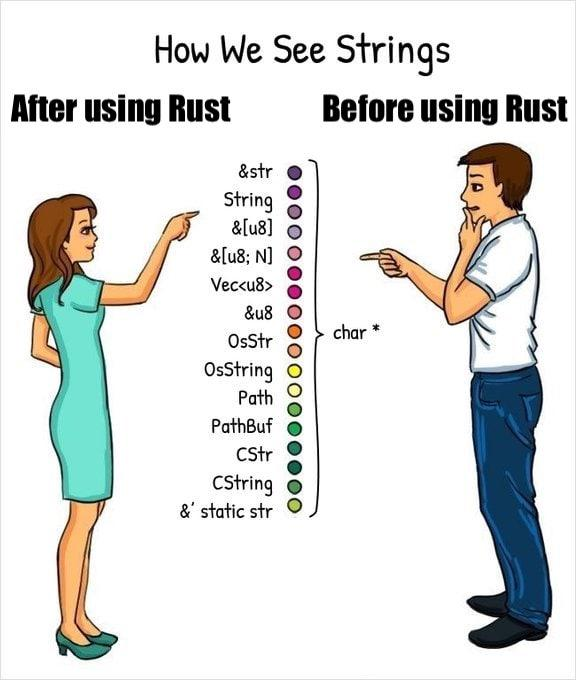
\includegraphics{img/strings.jpg}
\caption{strings}
\end{figure}

``Wow, what a mess, it's too complex! Better to use language like Go,
which is simpler.''

\textbf{You can't eliminate complexity. If it's not exposed, it's hidden
and may have unexpected consequences.}

\begin{itemize}
\tightlist
\item
  https://fasterthanli.me/articles/i-want-off-mr-golangs-wild-ride
\item
  https://viralinstruction.com/posts/defense/
\end{itemize}

also lol no generics
\end{frame}

\begin{frame}
How to make sense of this?

It's a common pattern that types in Rust are divided into ``owned''
types and ``borrowed'' types.
\end{frame}

\begin{frame}[fragile]
Owned types:

\begin{itemize}
\tightlist
\item
  \passthrough{\lstinline!String!} - Owned, Rust native, UTF-8 encoded,
  explicitly sized string
\item
  \passthrough{\lstinline!CString!} - Owned C-compatible null-terminated
  string
\item
  \passthrough{\lstinline!OsString!} - Owned, platform-native strings
  (so on Unix UTF-8, on Windows UTF-16, etc.)
\item
  \passthrough{\lstinline!PathBuf!} - Wrapper around
  \passthrough{\lstinline!OsString!}, with logic to manage path
  according to the platform (so on Unix separator is
  \passthrough{\lstinline!/!}, on Windows it's
  \passthrough{\lstinline!\\!}, etc.)
\item
  \passthrough{\lstinline!Vec<u8>!} - Owned vector of unsigned bytes
\end{itemize}
\end{frame}

\begin{frame}[fragile]
Borrowed types:

\begin{itemize}
\tightlist
\item
  \passthrough{\lstinline!\&str!}
\item
  \passthrough{\lstinline!\&' static str!}
\item
  \passthrough{\lstinline!CStr!}
\item
  \passthrough{\lstinline!OsStr!}
\item
  \passthrough{\lstinline!Path!}
\item
  \passthrough{\lstinline!\&[u8]!}
\item
  \passthrough{\lstinline!\&[u8; N]!}
\item
  \passthrough{\lstinline!\&u8!}
\end{itemize}
\end{frame}

\begin{frame}[fragile]
``But you told me borrowing in Rust is done with
\passthrough{\lstinline!\&!}, so why do some don't have that? Also, if
to borrow we just add \passthrough{\lstinline!\&!}, then why is borrowed
string not just \passthrough{\lstinline!\&String!}? What's the
difference?''
\end{frame}

\begin{frame}[fragile]{Strings}
\protect\hypertarget{strings}{}
To show the difference we'll look into just
\passthrough{\lstinline!\&str!} and \passthrough{\lstinline!String!}.

First, like any respectable programmer, let's turn for help to Stack
Overflow:

https://stackoverflow.com/questions/24158114/what-are-the-differences-between-rusts-string-and-str

\begin{figure}
\centering
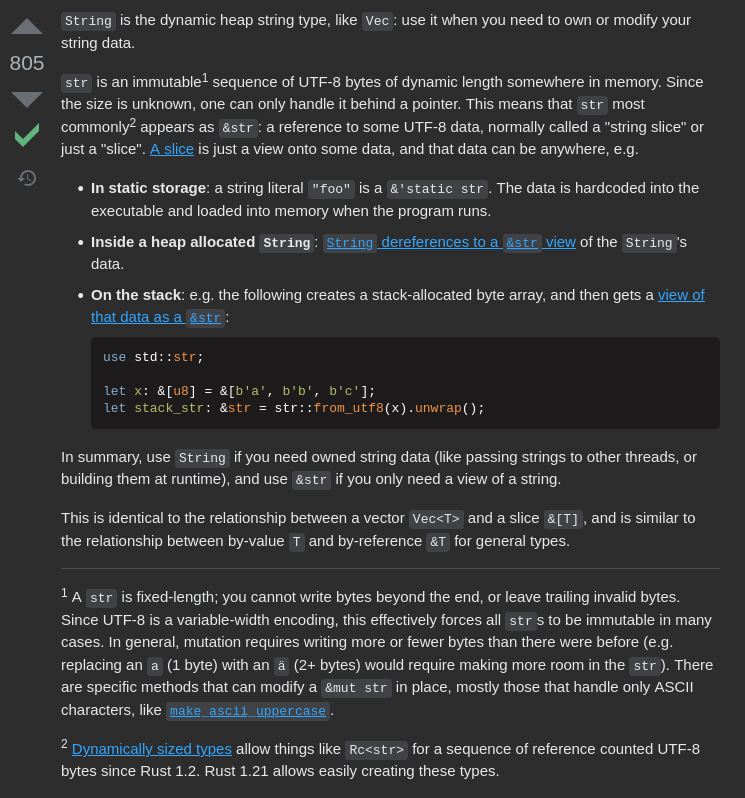
\includegraphics{img/string_str.png}
\caption{String vs str}
\end{figure}
\end{frame}

\begin{frame}[fragile]
\passthrough{\lstinline!String!}:

\begin{itemize}
\tightlist
\item
  Mutable
\item
  Manages memory
\item
  Heap-allocated
\end{itemize}

\passthrough{\lstinline!\&str!}:

\begin{itemize}
\tightlist
\item
  Immutable, ``view'' of the string
\item
  A reference to memory managed by somebody else - Is a ``slice'' so it
  can point to any portion of the string
\item
  Can be on heap, on stack, static, etc.
\end{itemize}
\end{frame}

\begin{frame}[fragile]
How they look on the inside?

In \emph{Rust pseudo-code}:

String:

\begin{lstlisting}
struct String {
    data: *mut u8,      // pointer to heap allocated data - 8 bytes
    length: usize,      // length of the string - 8 bytes
    capacity: usize,    // capacity of the string to grow, size of the current allocation - 8 bytes
}

dbg!(std::size_of::<String>()); // 24
\end{lstlisting}

Str:

\begin{lstlisting}
struct &str {
    data: *const u8 // pointer to string - 8 bytes
    length: usize   // length of the string - 8 bytes
}

dbg!(std::mem::size_of::<&str>()); // 16
\end{lstlisting}
\end{frame}

\begin{frame}[fragile]
So internally they're quite different, \passthrough{\lstinline!\&str!}
is smaller, and they do different things, that's why they are different
types. The same goes for the rest of types.

The following are analogous to \passthrough{\lstinline!String!} and
\passthrough{\lstinline!\&str!}:

\begin{itemize}
\tightlist
\item
  \passthrough{\lstinline!CString!} and \passthrough{\lstinline!CStr!}
\item
  \passthrough{\lstinline!OsString!} and \passthrough{\lstinline!OsStr!}
\item
  \passthrough{\lstinline!PathBuf!} and \passthrough{\lstinline!Path!}
\end{itemize}

More about strings:
https://fasterthanli.me/articles/working-with-strings-in-rust
\end{frame}

\begin{frame}[fragile]{Vecs and slices}
\protect\hypertarget{vecs-and-slices}{}
What about \passthrough{\lstinline!Vec<u8>!},
\passthrough{\lstinline![u8; N]!}, \passthrough{\lstinline!\&[u8; N]!},
\passthrough{\lstinline!\&[u8]!}?

\passthrough{\lstinline!Vec<u8>!} and \passthrough{\lstinline![u8; N]!}
are arrays of \passthrough{\lstinline!u8!}; former is growable and
heap-allocated, latter is constant size and may be on the stack.

\passthrough{\lstinline!\&[u8; N]!} - a reference to array of type
\passthrough{\lstinline!u8!} of size \passthrough{\lstinline!N!}

\passthrough{\lstinline!\&[u8]!} - a slice of type
\passthrough{\lstinline!u8!} (so, a ``view'' into an array of type
\passthrough{\lstinline!u8!}, either \passthrough{\lstinline!Vec<u8>!}
or \passthrough{\lstinline![u8; N]!})
\end{frame}

\begin{frame}[fragile]
``Ok, what does that mean for me, which should i use?''

In methods, use least restricive, most ``generic'' type:

Instead of:

\begin{lstlisting}
fn read_bytes(bytes: &Vec<u8>)
fn read_string(text: &String)
\end{lstlisting}

do:

\begin{lstlisting}
fn read_bytes(bytes: &[u8])
fn read_string(text: &str)
\end{lstlisting}
\end{frame}

\begin{frame}
But dont overthink it for now:

\begin{figure}
\centering

\includegraphics{img/api.jpg}
\caption{API}
\end{figure}
\end{frame}

\hypertarget{big-stdlib}{%
\subsection{Big stdlib}\label{big-stdlib}}

\begin{frame}[fragile]{Big stdlib}
Rust stdlib has two stdlibs:

\begin{itemize}
\tightlist
\item
  \passthrough{\lstinline!core!}, which is a subset of
  \passthrough{\lstinline!std!}, targets embedded, doesnt support
  allocation and shit
\item
  \passthrough{\lstinline!std!}, which is bigger, targets programs
  running on OSes that provide APIs for memory allocation, file
  operations, system calls, etc.
\end{itemize}
\end{frame}

\hypertarget{tooling-build-system-package-manager-rustfmt-clippy}{%
\subsection{Tooling (build system, package manager, rustfmt,
clippy)}\label{tooling-build-system-package-manager-rustfmt-clippy}}

\hypertarget{getting-started}{%
\section{Getting started}\label{getting-started}}

\hypertarget{how-install}{%
\subsection{How install?}\label{how-install}}

\begin{frame}{How install?}
Use rustup.rs. It lets you install multiple versions of rust. Usually
you'll use stable but sometimes you might want to use features that are
still unstable and available only on nightly. Also clippy and rustfmt
are parts of the toolchain.
\end{frame}

\hypertarget{linux}{%
\subsection{Linux}\label{linux}}

\begin{frame}[fragile]{Linux}
Install via your package manager or https://rustup.rs/ if it's not in
your distro's repositories. The website installer will automatically
prompt you to install the stable toolchain. If you installed rustup via
package manager, install stable toolchain:
\passthrough{\lstinline!rustup toolchain install stable!}.
\end{frame}

\hypertarget{windows}{%
\subsection{Windows}\label{windows}}

\begin{frame}{Windows}
Install via https://rustup.rs. To use MSVC backend, which is
recommended, you'll need to have installed either Visual Studio 2015+
C++ workload or VS C++ build tools standalone if you don't use visual
studio.

You can also use MinGW, but it won't be covered here.
\end{frame}

\hypertarget{ide-setup}{%
\subsection{IDE setup}\label{ide-setup}}

\begin{frame}{IDE setup}
I personally recommend VS Code with rust-analyzer, but feel free to use
something you're comfortable with if it's supported.

List of Rust IDEs/plugis available at: https://areweideyet.com

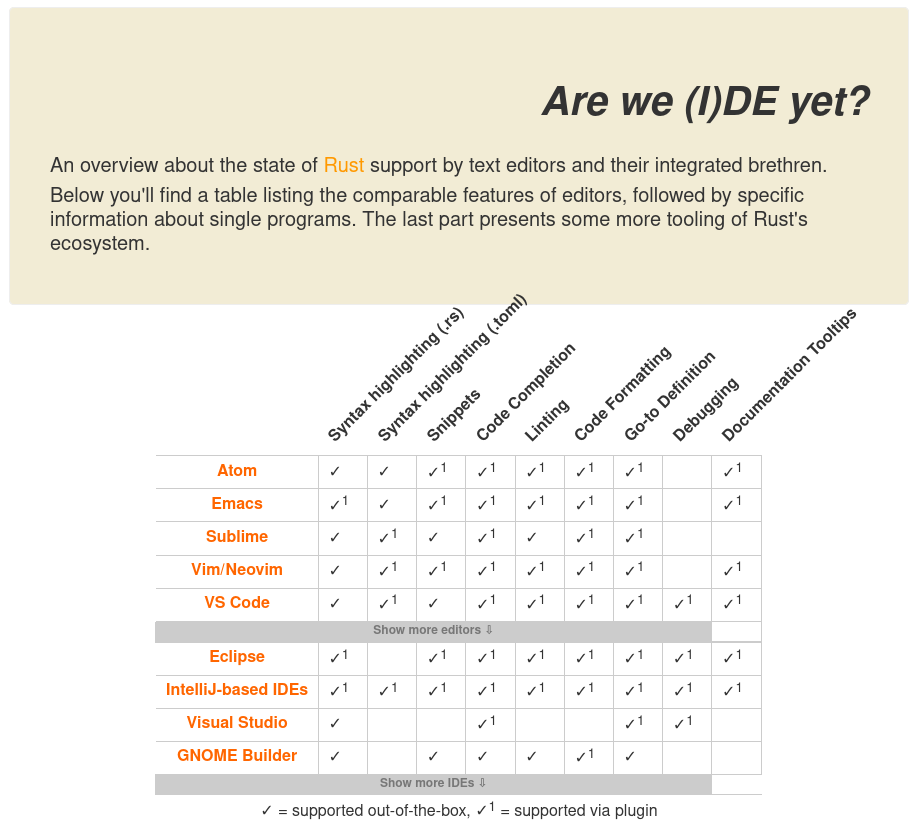
\includegraphics{img/ides.png}
\end{frame}

\hypertarget{vs-code-rust-analyzer}{%
\subsection{VS Code + rust-analyzer}\label{vs-code-rust-analyzer}}

\begin{frame}{VS Code + rust-analyzer}
What does rust-analyzer do?

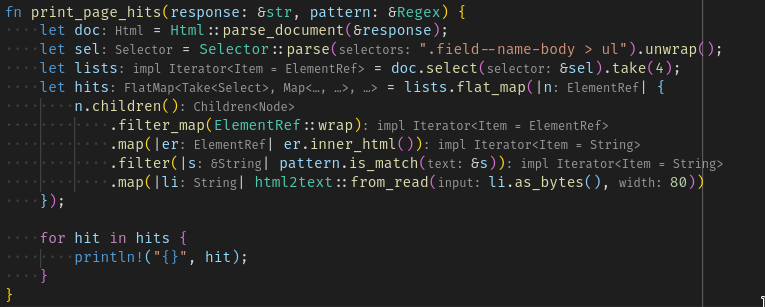
\includegraphics{img/ra1.png}

\begin{itemize}
\tightlist
\item
  type hinitng
\item
  autocomplete
\item
  jump to declaration/definition
\item
  Autoapply suggestions
\end{itemize}

After you have Rust stable toolchain installed, just install the VS Code
rust-analyzer extension. In case of difficulties, refer to the
\href{https://rust-analyzer.github.io/manual.html\#vs-code}{manual}.
\end{frame}

\hypertarget{troubleshooting}{%
\subsection{Troubleshooting}\label{troubleshooting}}

\begin{frame}[fragile]{Troubleshooting}
The extension works if the root directory of Rust project is opened in
VS Code (the folder that contains \passthrough{\lstinline!Cargo.toml!}).
If you have opened a directory with multiple Rust projects, you'll have
to manually specify paths for rust-analyzer.
\end{frame}

\hypertarget{learing-rust}{%
\section{Learing Rust}\label{learing-rust}}

\hypertarget{basics}{%
\subsection{Basics}\label{basics}}

\begin{frame}{Basics}
Basics of Rust
\end{frame}

\hypertarget{fearless-concurrency}{%
\subsection{Fearless concurrency}\label{fearless-concurrency}}

\begin{frame}{Fearless concurrency}
Sharing data between different threads
\end{frame}

\hypertarget{crates}{%
\subsection{Crates}\label{crates}}

\begin{frame}{Crates}
Crates
\end{frame}

\hypertarget{other-good-sources}{%
\subsection{Other good sources}\label{other-good-sources}}

\begin{frame}{Other good sources}
\begin{itemize}
\item
  \href{https://fasterthanli.me/articles/i-am-a-java-csharp-c-or-cplusplus-dev-time-to-do-some-rust}{I
  am a Java, C\#, C or C++ developer, time to do some Rust}

  Comprehensive introduction to Rust for developers of other Object
  Oriented languages
\item
  \href{https://fasterthanli.me/articles/declarative-memory-management}{Declarative
  memory management}

  How Rust memory management differs from C or C++
\item
  \href{https://learnxinyminutes.com/docs/rust/}{Learn Rust in Y
  minutes}
\item
  \href{https://doc.rust-lang.org/book/}{Rust Book}
\end{itemize}
\end{frame}

\hypertarget{other-tips}{%
\section{Other tips}\label{other-tips}}

\begin{frame}{Other tips}
\begin{itemize}
\tightlist
\item
  Use clone
\item
  Use clippy
\end{itemize}
\end{frame}

\hypertarget{sources}{%
\section{Sources}\label{sources}}

\begin{frame}{Sources}
\begin{itemize}
\tightlist
\item
  https://fasterthanli.me
\item
  https://www.youtube.com/c/fasterthanlime
\item
  https://www.youtube.com/c/JonGjengset
\item
  https://pkolaczk.github.io
\item
  https://www.reddit.com/r/rustjerk
\end{itemize}
\end{frame}

\end{document}
